\section{Principal Component Analysis}

Let
\[
\widetilde X=
\begin{bmatrix}
\widetilde x_1&\cdots&\widetilde x_N
\end{bmatrix},
\qquad
S=\frac{1}{N}\widetilde X\widetilde X^T
\]

\textbf{(a)}

\textbf{(i)}
The mean of the projected values \(v^Tx_i\) is \(v^T\bar x\), so their
centered values are \(v^T\widetilde x_i\). Their sample variance is
\[
\frac{1}{N}\sum_{i=1}^N(v^T\widetilde x_i)^2
=
v^T\left(\frac{1}{N}\sum_{i=1}^N
\widetilde x_i\widetilde x_i^T\right)v
=v^TSv
\]

\textbf{(ii)}
The covariance matrix is symmetric. For every \(z\),
\[
z^TSz
=\frac{1}{N}\|\widetilde X^Tz\|_2^2
\geq0
\]
so \(S\succeq0\). Using the full SVD
\[
\widetilde X=U\Sigma V^T
\]
gives
\[
S
=\frac{1}{N}U\Sigma\Sigma^TU^T
\]
Therefore the left singular vectors \(u_i\) are eigenvectors of \(S\), with
eigenvalues
\[
\boxed{\lambda_i=\frac{\sigma_i^2}{N}}
\]

\textbf{(iii)}
Expand a unit vector in the orthonormal eigenvector basis:
\[
v=\sum_i\alpha_i u_i,
\qquad
\sum_i\alpha_i^2=1
\]
Then
\[
v^TSv=\sum_i\lambda_i\alpha_i^2\leq\lambda_1
\]
Equality is attained at \(v=u_1\), so
\[
\boxed{\max_{\|v\|_2=1}v^TSv
=\lambda_1=\frac{\sigma_1^2}{N}}
\]

\textbf{(b)}

\textbf{(i)}
Let \(P=QQ^T\). Since
\[
\widehat x_i=\bar x+P\widetilde x_i
\]
we have
\[
x_i-\widehat x_i=(I-P)\widetilde x_i
\]
The vectors \(P\widetilde x_i\) and \((I-P)\widetilde x_i\) are orthogonal,
so the Pythagorean theorem gives
\[
\|\widetilde x_i\|_2^2
=\|P\widetilde x_i\|_2^2
+\|(I-P)\widetilde x_i\|_2^2
\]
Averaging over the data gives
\[
V=\frac{1}{N}\sum_i\|\widetilde x_i\|_2^2
=\frac{1}{N}\sum_i\|QQ^T\widetilde x_i\|_2^2+E(Q)
\]
Also,
\[
V
=\frac{1}{N}\operatorname{trace}(\widetilde X\widetilde X^T)
=\operatorname{trace}(S)
=\sum_i\lambda_i
\]

\textbf{(ii)}
The variance captured by the projection is
\[
\frac{1}{N}\sum_i\|QQ^T\widetilde x_i\|_2^2
=\operatorname{trace}(Q^TSQ)
\]
Thus
\[
E(Q)=\operatorname{trace}(S)-\operatorname{trace}(Q^TSQ)
\]
The lecture result for symmetric matrices states that
\(\operatorname{trace}(Q^TSQ)\) is maximized by
\[
Q=
\begin{bmatrix}
u_1&\cdots&u_k
\end{bmatrix}
\]
with value \(\lambda_1+\cdots+\lambda_k\). Therefore
\[
\boxed{E^\star
=\sum_{i>k}\lambda_i
=\frac{1}{N}\sum_{i>k}\sigma_i^2}
\]

\textbf{(c)}
% I centered the \(64\times1797\) data matrix and computed its SVD.

\textbf{(i)}
The first \(21\) principal components are needed to capture at least \(90\%\)
of the total variance.

\begin{figure}[H]
    \centering
    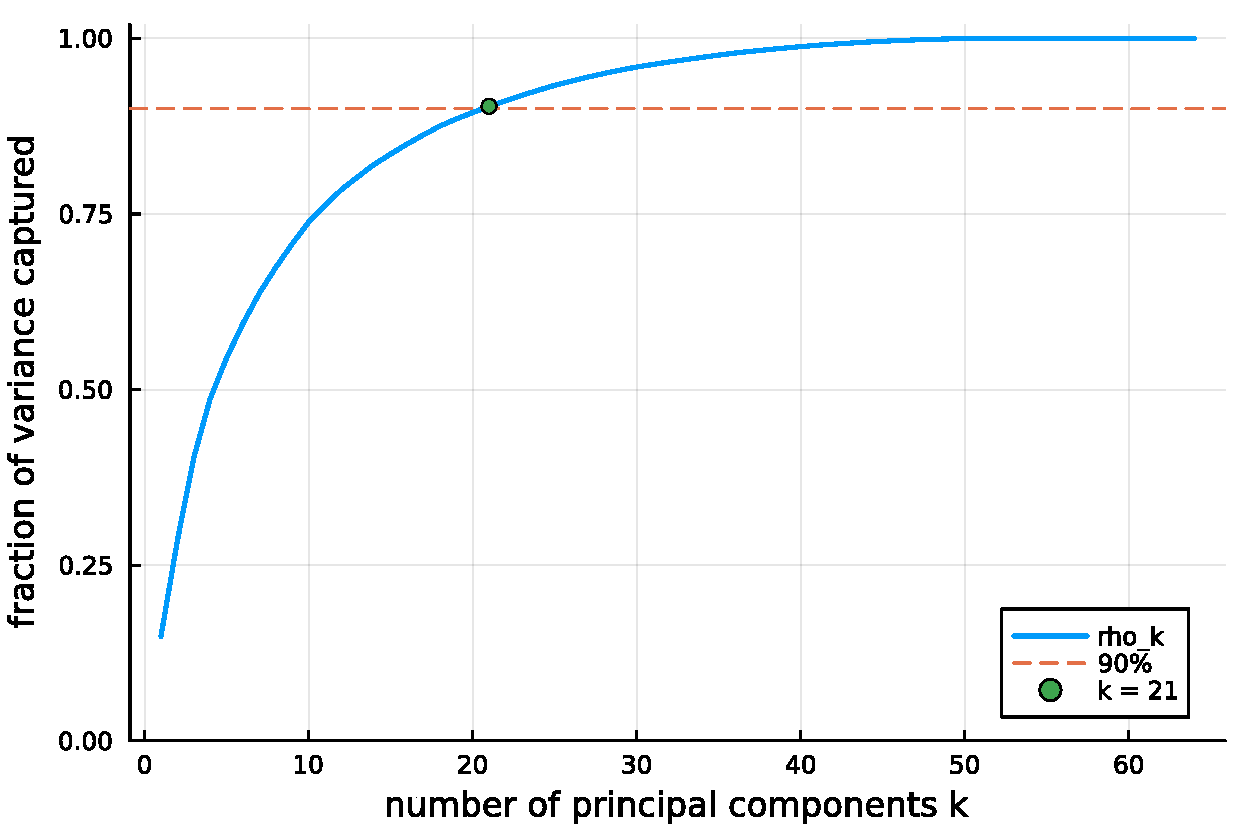
\includegraphics[width=0.78\textwidth]{img/p4_variance.pdf}
    % \caption{Cumulative fraction of variance captured}
\end{figure}

\textbf{(ii)}
The reconstructions below use the mean plus the projection onto the first
\(k\) principal components. With \(k=2\), substantial digit-specific detail is
lost. Around \(6\) components many digits are recognizable, and by \(12\)
components the displayed digits are clear. Thus roughly \(6\)--\(12\)
components are needed for recognizable reconstructions.

\begin{figure}[H]
    \centering
    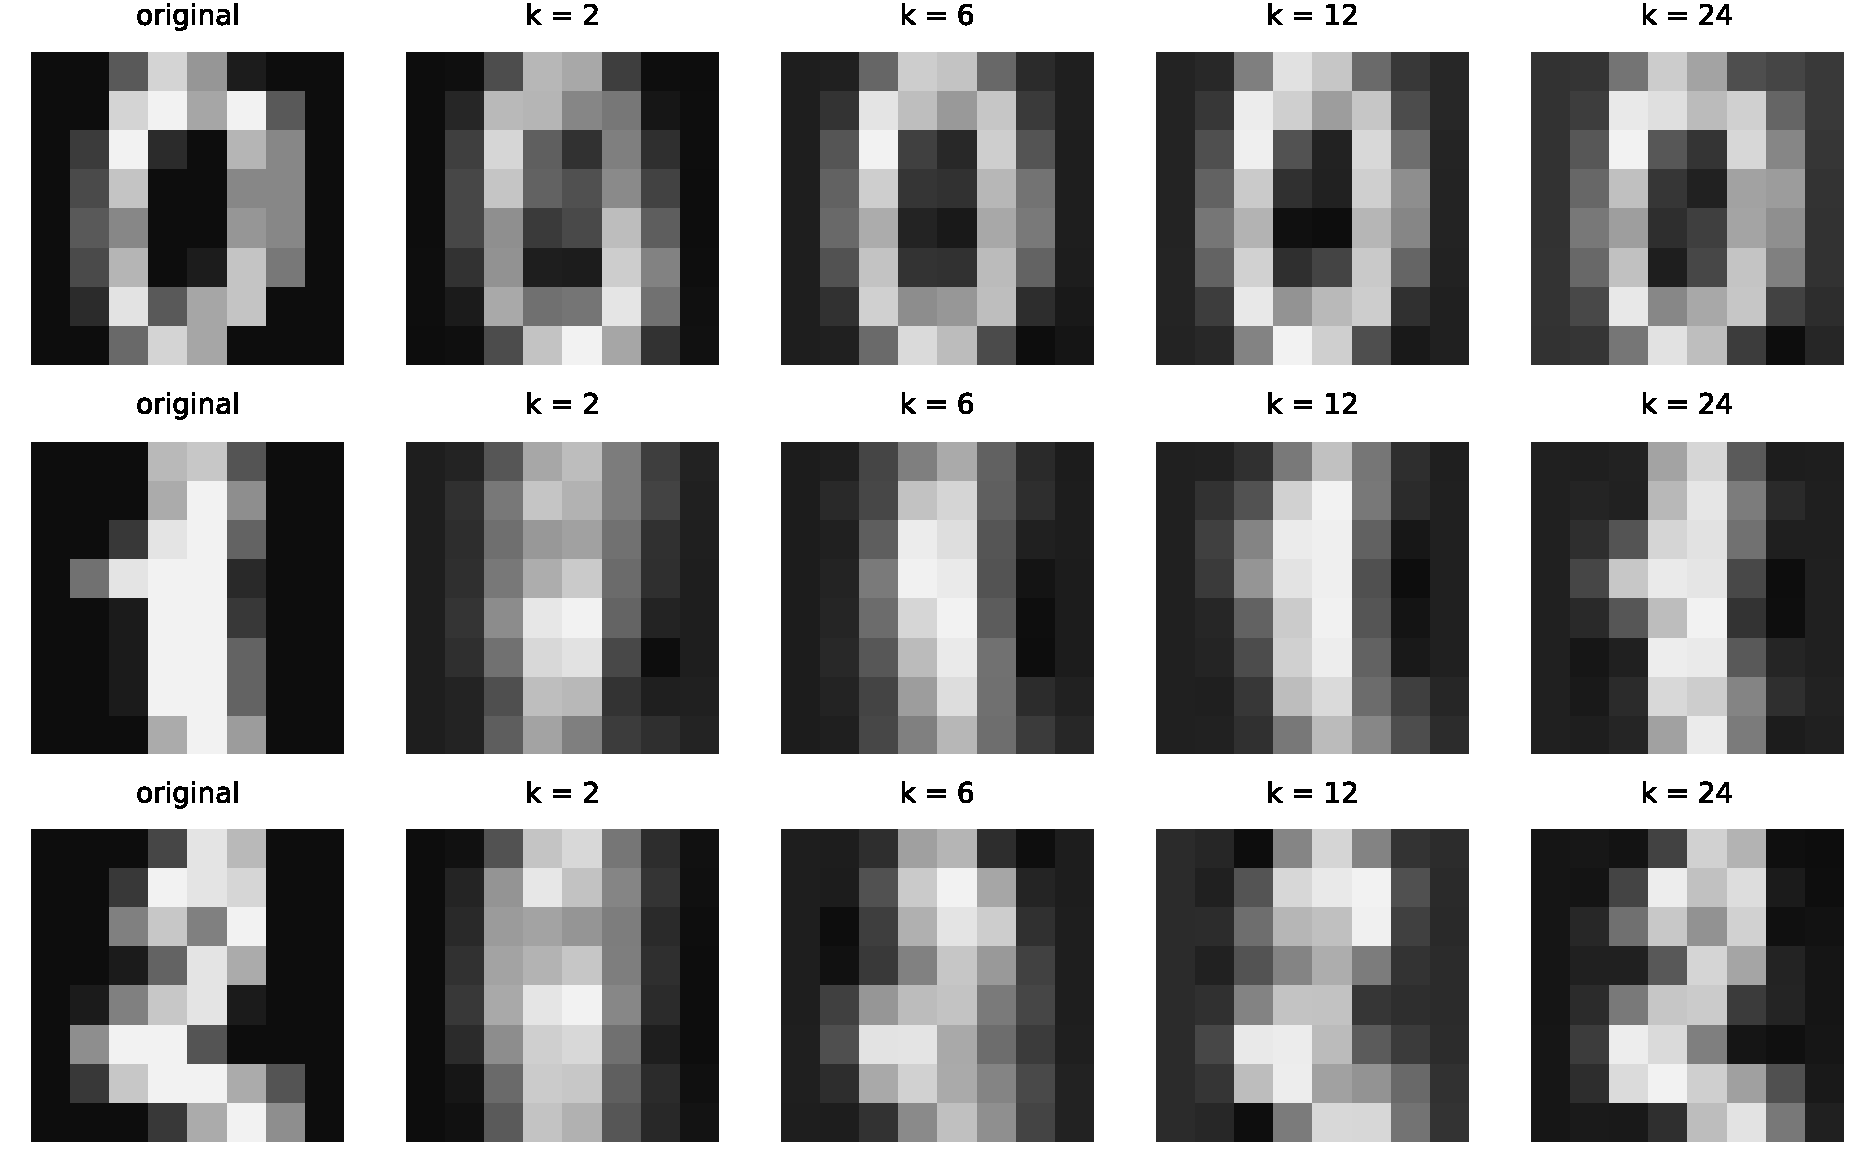
\includegraphics[width=\textwidth]{img/p4_reconstructions.pdf}
    % \caption{Original digits and PCA reconstructions}
\end{figure}

The mean image and first five principal components are shown below.

\begin{figure}[H]
    \centering
    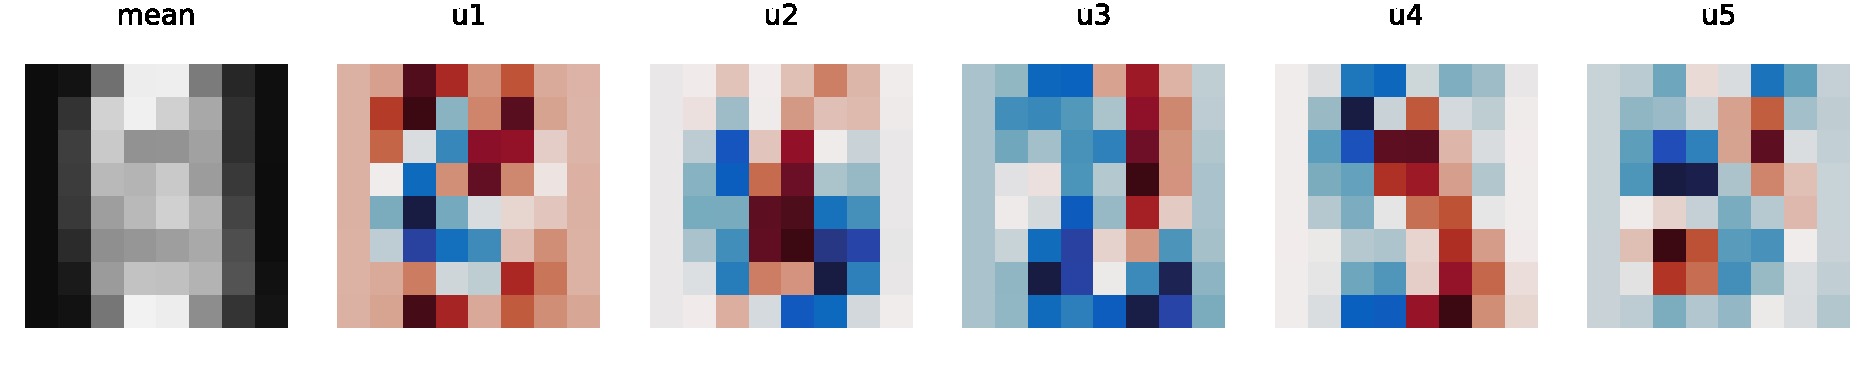
\includegraphics[width=\textwidth]{img/p4_components.pdf}
    % \caption{Mean image and leading principal components}
\end{figure}

\textbf{(iii)}
For \(k=10\), direct reconstruction gives
\[
\frac{1}{N}\sum_{i=1}^N\|x_i-\widehat x_i\|_2^2
=314.5149712423
\]
The discarded singular values give
\[
\frac{1}{N}\sum_{i>10}\sigma_i^2
=314.5149712423
\]
The absolute numerical difference is \(2.27\times10^{-13}\). The fraction of
total variance lost is
\[
1-\rho_{10}=0.261773
\]
so \(26.18\%\) of the variance is discarded.

\subsection{Code}
\begin{lstlisting}[language={},basicstyle=\ttfamily\footnotesize]
using LinearAlgebra
using Statistics
using Plots

include(joinpath(@__DIR__, "readclassjson.jl"))
data = readclassjson(joinpath(@__DIR__, "digits.json"))
X = data["X"]
n, N = size(X)

xbar = mean(X; dims=2)
Xc = X .- xbar
F = svd(Xc)

rho = cumsum(F.S .^ 2) ./ sum(F.S .^ 2)
k90 = findfirst(>=(0.90), rho)

plot(1:n, rho;
     xlabel="number of principal components k",
     ylabel="fraction of variance captured")
hline!([0.90]; linestyle=:dash)

function reconstruct(xc, k)
    Q = F.U[:, 1:k]
    return vec(xbar) + Q * (Q' * xc)
end

function digit_plot(x; title="")
    image = reshape(x, 8, 8)'
    return heatmap(image; color=:grays, yflip=true,
                   aspect_ratio=:equal, axis=false,
                   colorbar=false, title)
end

ks = [2, 6, 12, 24]
examples = [1, 2, 3]
panels = Any[]
for i in examples
    push!(panels, digit_plot(X[:, i]; title="original"))
    for k in ks
        xhat = reconstruct(Xc[:, i], k)
        push!(panels, digit_plot(xhat; title="k = $k"))
    end
end
plot(panels...; layout=(3, 5))

k = 10
Q = F.U[:, 1:k]
Xhat = xbar .+ Q * (Q' * Xc)
empirical_error = norm(X - Xhat)^2 / N
predicted_error = sum(F.S[(k + 1):end] .^ 2) / N
\end{lstlisting}
